\documentclass[11pt]{article}

\usepackage[margin=1in, headheight=14.5pt]{geometry}
\usepackage{amsfonts, amsmath, amssymb}
\usepackage{enumitem}
\usepackage[none]{hyphenat}
\usepackage{fancyhdr}
\usepackage[spanish, es-noshorthands]{babel}
\usepackage[spanish, calc]{datetime2}
\usepackage{fmtcount}
\usepackage{graphicx}
\usepackage{float}
\usepackage[nottoc, notlot, notlof]{tocbibind}
\usepackage{tocloft}
\usepackage[utf8]{inputenc}
\usepackage{parskip}
\usepackage{xcolor}
\usepackage{cancel}
\usepackage{textcomp}
\usepackage{pgfplots}
\usepackage{tikz}
\usetikzlibrary{shapes.misc}
\usepackage{polynom}
\usetikzlibrary{datavisualization}
\usetikzlibrary{datavisualization.formats.functions}
\pgfplotsset{compat=1.15}
\usepackage{mathrsfs}
\usetikzlibrary{arrows}

\newcommand{\dropsign}[1]{\smash{\llap{\raisebox{-.5\normalbaselineskip}{$#1$\hspace{2\arraycolsep}}}}}%


\parindent 0ex

\pgfplotsset{width=10cm,compat=1.9}

\def\imj{\mathrm{j}}
\def\sen{\mathrm{sen}}

\newcommand{\lapl}[1]{\mathscr{L} \left\lbrace {#1} \right\rbrace}
\newcommand{\ilapl}[1]{\mathscr{L}^{-1} \left\lbrace {#1} \right\rbrace}

\renewcommand\cftsecleader{\cftdotfill{\cftdotsep}}
\renewcommand{\baselinestretch}{1.1}
\newcommand*\circled[1]{\tikz[baseline=(char.base)]{
		\node[shape=circle,draw,inner sep=2pt] (char) {#1};}}
	
\newcommand{\highlight}[2]{\colorbox{#1}{$\displaystyle #2$}}

\graphicspath{{\ProjectRoot/commons/img/}}

\newcommand*{\ProjectRoot}{../../matematica-superior}


\begin{document}
		
	\begin{titlepage}
		\begin{center}
			\vspace*{0.5cm}
			\Large{\textbf{Universidad Tecnológica Nacional}}\\
			\Large{\textbf{Facultad Regional Buenos Aires}}\\
			\begin{center}
				
\includegraphics[scale=0.4]{logoutn.png}
			\end{center}
			\vfill
			\line(1,0){400}\\
			\vspace*{0.3cm}
			\huge{\textbf{Matemática Superior}}\\
			\Large{\textbf{Unidad 4: Función Transferencia y Sistemas Estables}}\\
			\large{Ejercicios resueltos}
			\line(1,0){400}\\
			\vfill
			Tomás Moreira \\
			
			\DTMnewdatestyle{mydate}{%
				\renewcommand{\DTMdisplaydate}[4]{%
					\DTMMonthname{##2} \number##1
				}
				\renewcommand{\DTMDisplaydate}{\DTMdisplaydate}
			}
			
			\DTMsetdatestyle{mydate}
			\today
				
				
		\end{center}
	\end{titlepage}

	\tableofcontents
	\thispagestyle{empty}
	\clearpage

	\setcounter{page}{1}
	
	\section{Parte 1: Función transferencia - Polos y ceros}
	\subsection{Ejercicio 3}
	Sea $\displaystyle G(s)=\frac{k(s^2-4s-5)}{s^3-3s^2-25s+75}$ la transferencia de un sistema.
	\begin{enumerate}[label=(\alph*)]
		\item Grafique la constelación de polos y ceros de $G(s)$.
		\item Halle $k \in \mathbb{R}^{+} / \; |G(\imj)|=1$
		\item Grafique \underline{aproximadamente} $|G(s)|$ a lo largo del eje $\sigma=\text{Re}(s)$
	\end{enumerate}

	Empezamos con nueva unidad. Esta tiene la particularidad de ser integradora de Números Complejos y Transformada de Laplace.
	
	Una función transferencia, por lo general, se usa para representar sistemas, y relaciona la entrada y la salida del mismo.
	
	Si tenemos que $X(s)$ es la entrada y que $Y(s)$ es la salida (o respuesta) del sistema, entonces la función transferencia es:
	
	$\displaystyle G(s)=\frac{Y(s)}{X(s)}$
	
	Hay que tener en cuenta que tanto $X$ como $Y$ son polinomios de variable compleja con \fcolorbox{white}{yellow}{coeficientes reales}.
	
	En forma genérica: $\displaystyle G(s)=\frac{a_0+a_1s+a_2s^2+\dots+a_ns^n}{b_0+b_1s+b_2s^2+\dots+b_ms^m}=\frac{a_n(s-z_1)(s-z_2)\dots(s-z_n)}{b_m(s-p_1)(s-p_2)\dots(s-p_m)}$
	
	En donde $n<m$
	
	De forma resumida, podemos escribir a $G$ como: $\displaystyle G(s)=k\frac{\prod (s-z_i)}{\prod(s-p_j)}$, donde $k=\frac{a_n}{b_m}$
	
	Los ``$z$'' los vamos a llamar ceros de la función, mientras que los ``$p$'' son los polos de la función.
	
	\begin{itemize}
		\item $z$ es un cero de $G$ si cumple: $\displaystyle \lim\limits_{s\rightarrow z_i}=0$
		\item $p$ es un polo de $G$ si cumple: $\displaystyle \lim\limits_{s\rightarrow p_j}=\infty$
	\end{itemize}

	Con este breve repaso, vamos a encarar la solución del ejercicio.
	
	Primero, vamos a factorizar a $G$:
	
	$\displaystyle G(s)=k\frac{\cancel{(s-5)}(s+1)}{(s+5)\cancel{(s-5)}(s-3)}=k\frac{(s+1)}{(s-3)(s+5)}$
	
	Los ceros de $G$ son:
	\begin{itemize}
		\item $z_1=-1$
		\item $z_2=\infty$
	\end{itemize}

	Sus polos:
	\begin{enumerate}[label=(\alph*)]
		\item $p_1=3$
		\item $p_2=-5$
	\end{enumerate}

	La constelación entonces es:
	
	\begin{tikzpicture}
		\draw [-latex] (-6,0) -- (4,0) node [below right] {$\sigma$};
		\draw [-latex] (0,-1) -- (0,1) node [below right] {$\text{j} \omega$};
		
		\node[label=below:{3}, cross out, draw=black] at (3,0) {};
		\node[label=below:{-5}, cross out, draw=black] at (-5,0) {};
		\node[label=below:{-1}, circle, draw=black] at (-1,0) {};
	\end{tikzpicture}

	Vamos ahora con el inciso b.
	
	Hay que calcular el $|G(\imj)|$. Hacemos eso:
	
	$\displaystyle |G(\imj)|=|k|\frac{|\imj+1|}{|\imj-3||\imj+5|} \rightarrow 1=k\frac{\sqrt{2}}{\sqrt{10}\sqrt{26}}\rightarrow k=\frac{\sqrt{10} \sqrt{26}}{\sqrt{2}}\rightarrow$ \fcolorbox{black}{yellow}{$k=\sqrt{130}$}
	
	Por último, hacemos el gráfico de $|G(s)|$:\\
	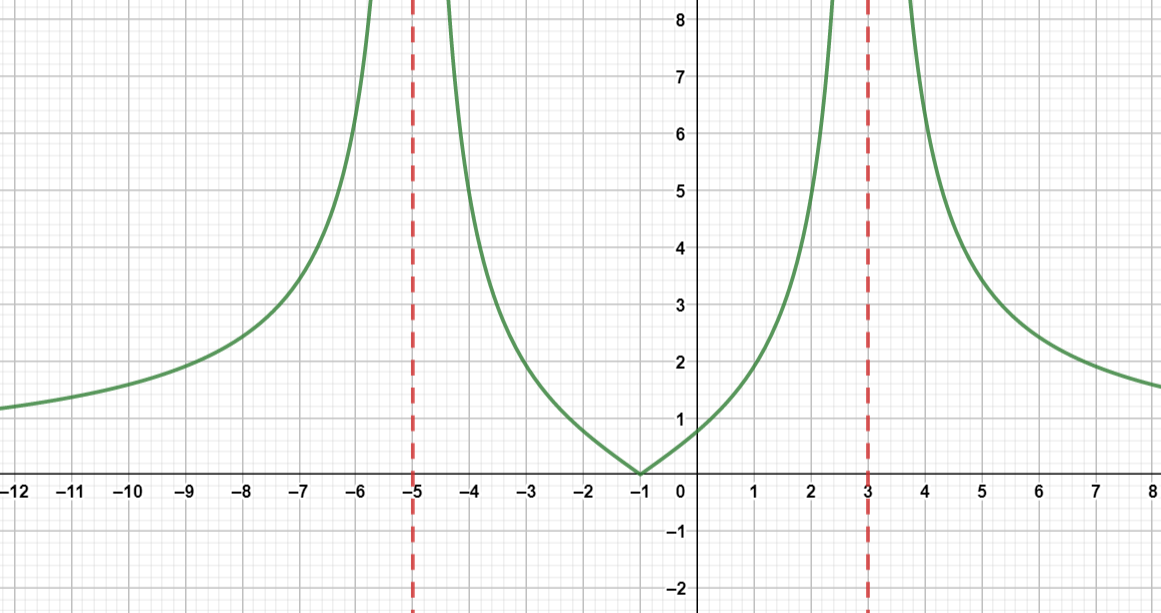
\includegraphics[scale=0.6]{04-FuncionTransferenciaYSistemasEstables/3.png}
	
	\subsection{Ejercicio 4}
	
	Sea $\displaystyle G(s)=\frac{s(s+2)}{s^3+2s^2+9s+k}$ la transferencia de un sistema.
	\begin{enumerate}[label=(\alph*)]
		\item Halle $k \in \mathbb{R}$ sabiendo que $3\imj$ es un polo.
		\item Grafique aproximadamente $|G(\imj \omega)|$
	\end{enumerate}

	Para el inciso a, si $3\imj$ es polo, quiere decir que el denominador evaluado en $3\imj$ da cero:
	
	$(3\imj)^3+2(3\imj)^2+9\cdot 3\imj+k=0 \rightarrow -27\imj -18 + 27\imj + k = 0 \rightarrow$ \fcolorbox{black}{yellow}{$k=18$}
	
	Quedando $\displaystyle G(s)=\frac{s(s+2)}{s^3+2s^2+9s+18}=\frac{s\cancel{(s+2)}}{\cancel{(s+2)}(s^2+9)}=\frac{s}{s^2+9}$
	
	Con esta última $G$, hacemos el inciso b:\\
	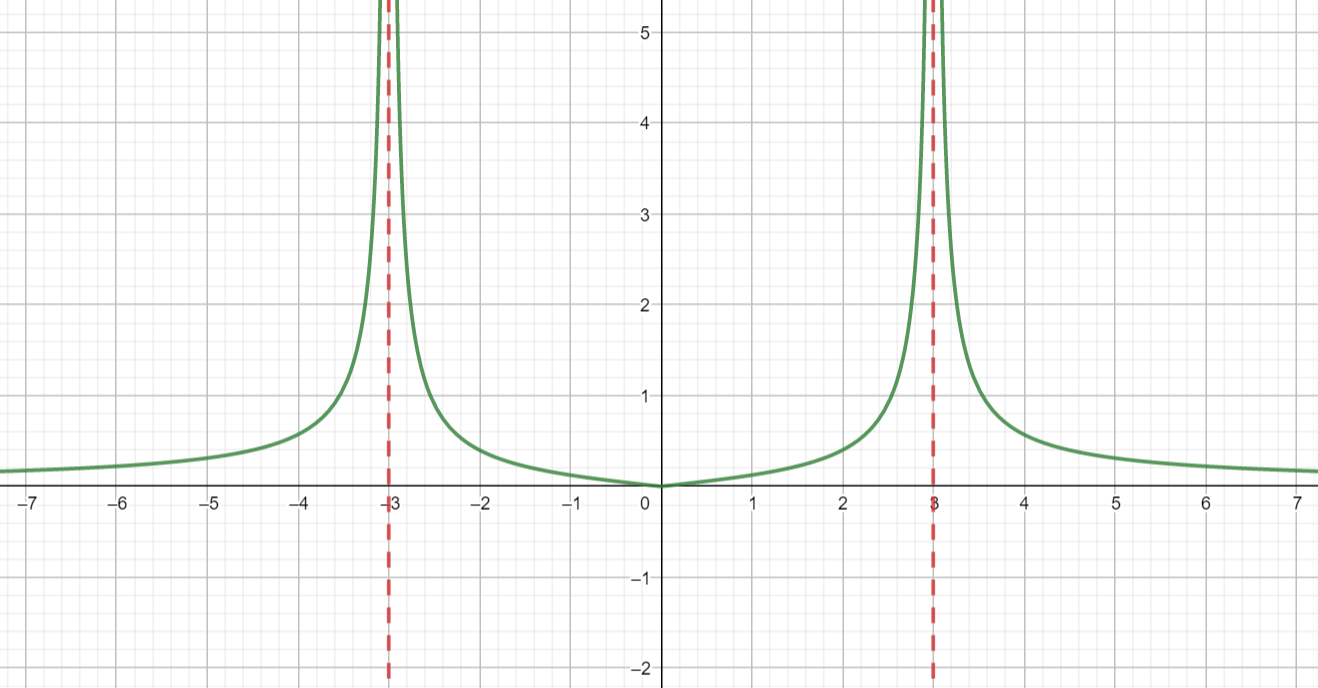
\includegraphics[scale=0.6]{04-FuncionTransferenciaYSistemasEstables/4.png}
	
	\subsection{Ejercicios 6bi}
	Construya funciones de transferencia que cumplan los siguientes requisitos:
	
	
	\subsubsection{6b}
	cuya constelación de polos y ceros sea la de la figura y $G(0)=-2$:
	
	\begin{tikzpicture}
		\draw [-latex] (-5,0) -- (5,0) node [below right] {$\sigma$};
		\draw [-latex] (0,-4) -- (0,4) node [below right] {$\text{j} \omega$};
		
		\draw [dashed] (-3,0) node[below] {$-3$} -- (-3, 1) node[solid, circle, draw=black] {};
		\draw [dashed] (-3,0) node[below] {} -- (-3, -1) node[solid, circle, draw=black] {};
		\draw [dashed] (-3,1) -- (0, 1) node[right]{$\imj$};
		\draw [dashed] (-3,-1) -- (0, -1) node[right]{$-\imj$};
		
		\draw [dashed] (-2,0) node[below] {$-2$} -- (-2, 3) node[solid, cross out, draw=black] {};
		\draw [dashed] (-2,0) node[below] {} -- (-2, -3) node[solid, cross out, draw=black] {};
		\draw [dashed] (-2,3) -- (0, 3) node[right]{$3\imj$};
		\draw [dashed] (-2,-3) -- (0, -3) node[right]{$-3\imj$};
		
		\node[label=below:{1}, cross out, draw=black] at (1,0) {};
	\end{tikzpicture}

	De la constelación podemos saber que:\\
	$z_1=-3+\imj \;;\; z_2=-3-\imj$\\
	$p_1=-2+3\imj \;;\; p_2=-2-3\imj \; ; \; p_3=1$
	
	Antes de continuar, vamos a deducir una especie de formulita que nos va a ayudar a expresar una factorización por raíces complejas conjugadas a la forma polinómica:
	
	$(s-(a+b\imj))\cdot(s-(a-b\imj))=(s-a-b\imj)\cdot(s-a+b\imj)=s^2-as+\cancel{bs\imj}-as+a^2-\cancel{ab\imj}-\cancel{bs\imj}+\cancel{ab\imj}+b^2$\\
	$= \boxed{s^2 -2as +a^2+b^2}$
	
	Usando esta especie de identidad, podemos expresar de forma muy sencilla en forma polinómica los ceros y polos que tenemos:
	
	$\displaystyle G(s)=k\frac{s^2-2\cdot(-3)\cdot s+(-3)^2+1^2}{(s-1)(s^2-2\cdot(-2)\cdot s+(-2)^2+3^2)}=k\frac{s^2+6s+10}{(s-1)(s^2+4s+13)}$
	
	Ahora, usamos el dato $G(0)=-2$ para hallar el valor de $k$:
	
	$\displaystyle -2=k\frac{0^2+6\cdot0+10}{(0-1)(0^2+4\cdot0+13)} \rightarrow k=\frac{26}{10} \rightarrow$ \fcolorbox{black}{yellow}{$\displaystyle k=\frac{13}{5}$}
	
	Por último, nuestra función queda: \fcolorbox{black}{yellow}{$\displaystyle G(s)=\frac{\frac{13}{5}(s^2+6s+10)}{(s-1)(s^2+4s+13)}$}
	
	\subsubsection{6i}
	sabiendo que $G(0)=3\text{, }G(1)=5$ y el corte de la misma con el eje real es:\\
	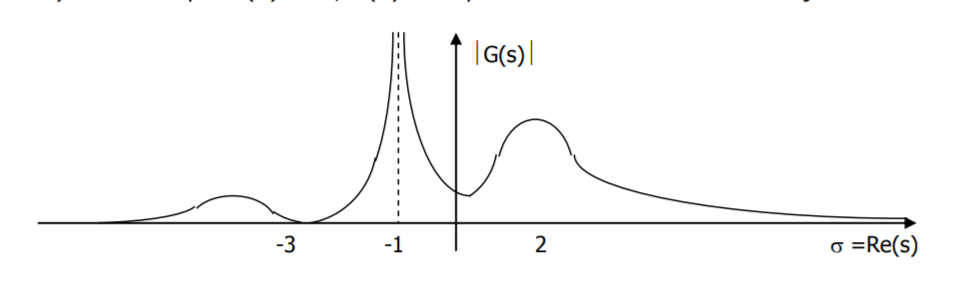
\includegraphics[scale=0.8]{04-FuncionTransferenciaYSistemasEstables/6i.png}
	
	A simple vista podemos identificar:\\
	$z_1=-3 \;;\; p_1=-1$
	
	Y luego, la ``pancita'' que hay en el $2$ indica la presencia de un par de polos complejos conjugados. Notar que esta pancita es más considerablemente más alta que la que está al costado del $-3$, siendo esta solo un rebote de la función con el eje, para dar continuidad a la gráfica. Por ende, tenemos otro dato más:
	
	$p_2=2+a\imj \;;\;p_3=2-a\imj$
	
	Expresamos estos polos como polinomio: $s^2-4s+4+a^2$
	
	$\displaystyle G(s)=k\frac{s+3}{(s+1)(s^2-4s+4+a^2)}$
	
	Usamos los datos que nos dan en el ejercicio para despejar las incógnitas:
	
	$\displaystyle \cancel{3}=k\frac{\cancel{3}}{4+a^2} \rightarrow k=4+a^2$\\
	$\displaystyle 5=k\frac{4}{2(1-4+4+a^2)} \rightarrow 5=\frac{4(4+a^2)}{2(1+a^2)} \rightarrow 5+5a^2=8+2a^2 \rightarrow \boxed{a^2=1}$
	
	Usando el cálculo $a^2=1$ podemos calcular $k$ de la primera ecuación: $k=5$
	
	Por último, \fcolorbox{black}{yellow}{$\displaystyle G(s)=\frac{5(s+3)}{(s+1)(s^2-4s+5)}$}
	
	\section{Parte 2: Respuesta de sistemas}
	\subsection{Ejercicio 10}
	Sea $\displaystyle G(s)=\frac{3s^2-6s-24}{s^3-3s^2-4s}$ la transferencia de un sistema.
	
	\begin{enumerate}[label=(\alph*)]
		\item Grafique la constelación de polos y ceros de $G(s)$ e indique si el sistema es estable.
		\item Halle módulo y fase de $G(-1+\imj)$ por el método gráfico y por método analítico.
		\item ¿Cuál será la respuesta del sistema si se lo excita con una señal $v_1(t)=e^{-t}$?
	\end{enumerate}

	Para el inciso a, primero factoreamos a $G$:
	
	$\displaystyle G(s)=\frac{3\cancel{(s-4)}(s+2)}{s\cancel{(s-4)}(s+1)}=\frac{3(s+2)}{s(s+1)}$
	
	La constelación es entonces:
	
	\begin{tikzpicture}
		\draw [-latex] (-4,0) -- (2,0) node [below right] {$\sigma$};
		\draw [-latex] (0,-2) -- (0,2) node [below right] {$\text{j} \omega$};
		
		\node[label=below:{-2}, circle, draw=black] at (-2,0) {};
		\node[label=below:{-1}, cross out, draw=black] at (-1,0) {};
		\node[label=below:{0}, cross out, draw=black] at (0,0) {};
	\end{tikzpicture}

	La representación de esta constelación nos lleva a concluir que el sistema es estable.\\
	
	Inciso b:
	
	Por el método gráfico tenemos que hacer lo siguiente:
	
	\begin{tikzpicture}
		\draw [-latex] (-4,0) -- (2,0) node [below right] {$\sigma$};
		\draw [-latex] (0,-2) -- (0,2) node [below right] {$\text{j} \omega$};
		
		\node[label=below:{-2}, circle, draw=black] at (-2,0) {};
		\node[label=below:{-1}, cross out, draw=black] at (-1,0) {};
		\node[label=below:{0}, cross out, draw=black] at (0,0) {};
		\node[label=above:{$-1+\imj$}, circle, draw=black, fill=black, very thin] at (-1, 1) {};
		
		\draw [->, cyan] (-2,0) -- (-1,1) node [below right] {};
		\draw [->, red] (-1,0) -- (-1,1) node [below right] {};
		\draw [->, red] (0,0) -- (-1,1) node [below right] {};
	\end{tikzpicture}

	Graficamos el punto en cuestión en la constelación, y luego unimos los polos y ceros con el punto, con vectores.
	
	A continuación se hace uso de las fórmulas:
	
	$\displaystyle |G(s)|=k\frac{\prod \text{módulos vectores origen ceros}}{\prod \text{módulos vectores origen polos}}$
	
	$\displaystyle \text{Arg}[G(s)]=\sum \text{args de vectores con origen en ceros} - \sum \text{args de vectores con origen en polos}$
	
	$\displaystyle |G(s)|=\frac{3}{1} \cdot \frac{\sqrt{2}}{1\cdot \sqrt{2}}=$\fcolorbox{black}{yellow}{$3$}
	
	Luego, para el argumento hay que tener en cuenta que se toma el semieje real positivo como punto de partida. De esta manera, tenemos:
	
	$\displaystyle \text{Arg}[G(-1+\imj)]= \frac{\pi}{4} - \left(\frac{\pi}{2} + \frac{3}{4}\pi \right)=$ \fcolorbox{black}{yellow}{$-\pi$}\\
	
	Para hacerlo de forma analítica:
	
	$\displaystyle |G(-1+\imj)|=\frac{3|-1+\imj+2|}{|-1+\imj||-1+\imj+1|}=\frac{3|1+\imj|}{|-1+\imj||\imj|}=\frac{3 \cdot \sqrt{2}}{\sqrt{2} \cdot 1} \rightarrow$ \fcolorbox{black}{yellow}{$|G(-1+\imj)|=3$}
	
	$\displaystyle G(-1+\imj)=\frac{3(-1+\imj+2)}{(-1+\imj)(-1+\imj+1)}=\frac{3(1+\imj)}{(-1+\imj)\imj}=\frac{3+3\imj}{-1-\imj}\cdot\frac{-1+\imj}{-1+\imj}=\frac{-6}{2}=-3$
	
	Le calculamos el argumento a este último número: \fcolorbox{black}{yellow}{$\displaystyle \arctan\left(\frac{0}{-3}\right) + \pi=\pi$}
	
	Los resultados concuerdan, ya que $-\pi$ es congruente con $\pi$.\\
	
	Por último, para el inciso c:
	
	Recordemos que la función transferencia es $\displaystyle G(s)=\frac{Y(s)}{X(s)}$, con $X$ siendo la entrada e $Y$ siendo la salida. Estas funciones $X$ e $Y$ son la Transformada de Laplace de una función $x(t)$ e $y(t)$, respectivamente!
	
	\textbf{\underline{IMPORTANTE:}} tener en cuenta que $\displaystyle G(s)=\frac{Y(s)}{X(s)}$, pero $\displaystyle g(t)\neq\frac{y(t)}{x(s)}$. Esto es un error conceptual muy grave. La división es válida en el dominio de Laplace.
	
	Con estas consideraciones, transformamos la entrada: $\displaystyle \lapl{v_1(t)}=V_1(t)=\frac{1}{s+1}$
	
	Dado que $\displaystyle G(s)=\frac{Y(s)}{X(s)}$, entonces: $\displaystyle Y(s)=X(s)\cdot G(s)$ (en este caso $X$ es $V_1$)
	
	Entonces $\displaystyle Y(s)=\frac{1}{s+1} \cdot \frac{3(s+2)}{s(s+1)}=\frac{3(s+2)}{s(s+1)^2}$
	
	Aplicando fracciones simples queda (no nos vamos a detener en esto, puesto que lo vimos en la unidad pasada):
	
	$\displaystyle Y(s)=\frac{6}{s}-\frac{3}{(s+1)^2}-\frac{6}{s+1}$
	
	Por último, antitransformamos para obtener la respuesta:
	
	\fcolorbox{black}{yellow}{$y(t)=6-3te^{-t}-6e^{-t}$}
	
	\subsection{Ejercicio 12}
	Sea $\displaystyle G(s)=\frac{2(s^2-5s-6)}{s^3-6s^2+4s-24}$ la transferencia de un sistema.
	
	\begin{enumerate}[label=(\alph*)]
		\item De acuerdo a la constelación de polos y ceros, indique si el sistema es estable.
		\item ¿Cuál será la respuesta del sistema al escalón unitario $E(t)$?
	\end{enumerate}

	Primero factorizamos:
	
	$\displaystyle G(s)=\frac{2\cancel{(s-6)}(s+1)}{\cancel{(s-6)}(s^2+4)}=\frac{2(s+1)}{s^2+4}$
	
	Ahora, hacemos el inciso a:
	
	\begin{tikzpicture}
		\draw [-latex] (-3,0) -- (2,0) node [below right] {$\sigma$};
		\draw [-latex] (0,-3) -- (0,3) node [below right] {$\text{j} \omega$};
		
		\node[label=right:{$2\imj$}, cross out, draw=black] at (0,2) {};
		\node[label=right:{$-2\imj$}, cross out, draw=black] at (0,-2) {};
		\node[label=below:{$-1$}, circle, draw=black] at (-1,0) {};
	\end{tikzpicture}

	Con esta constelación, decimos que el sistema es estable, particularmente MARGINALMENTE estable, porque tiene polos sobre el eje imaginario.\\
	
	Inciso b:
	
	$\displaystyle Y(s)=X(s)\cdot G(s)=\frac{1}{s}\cdot \frac{2(s+1)}{s^2+4}=\frac{2(s+1)}{s(s^2+4)}$
	
	Aplicando fracciones simples:
	
	$\displaystyle Y(s)=\frac{\frac{1}{2}}{s}+\frac{-\frac{1}{2}s}{s^2+4}+\frac{2}{s^2+4}$
	
	Antitransformando:
	
	\fcolorbox{black}{yellow}{$\displaystyle y(t)=\frac{1}{2}-\frac{1}{2} \cos(2t) + \sen(2t)$}
	
	\section{Parte 3: Problemas aplicados}
	\subsection{Ejercicio 15}
	Sea el sistema mecánico de la figura, que parte del reposo:\\
	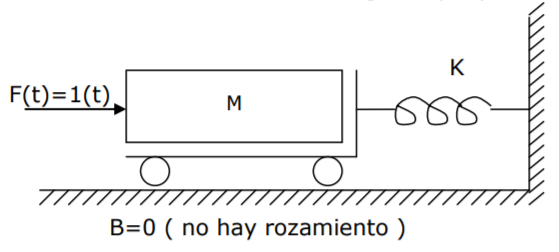
\includegraphics[scale=0.75]{04-FuncionTransferenciaYSistemasEstables/carrito15.png}\\
	Hallar:
	\begin{enumerate}[label=(\alph*)]
		\item La ecuación diferencial correspondiente al movimiento $x(t)$ del sistema.
		\item La función de transferencia del sistema.
		\item La expresión de $x(t)$ considerando $M=1 \wedge K=9$
	\end{enumerate}

	Inciso a:
	
	No hay que tener miedo en estos ejercicios! Primero, la ecuación diferencial que vamos a hallar ahora SUELE ser dato en los exámenes. Segundo, hay que recordar Física I un ratito nada más.
	
	Usamos la Segunda Ley de Newton:
	
	$\sum F=M\cdot a(t)$
	
	Las fuerzas que interactúan en el sistema son:
	\begin{itemize}
		\item La fuerza externa $f(t)$.
		\item La fuerza amortiguadora $B\cdot v(t)$.
		\item La fuerza del resorte $K \cdot x(t)$.
	\end{itemize}

	Entonces, planteamos:
	$f(t)-Kx(t)-Bv(t)=Ma(t)$
	
	Pero sabemos que la velocidad es la derivada primera respecto del tiempo de la posición. Lo mismo para la aceleración, solo que esta es la derivada segunda, entonces queda finalmente planteada la ecuación diferencial:
	
	\fcolorbox{black}{yellow}{$f(t)-Kx(t)-Bx'(t)=Mx''(t)$}\\
	
	Inciso b:
	
	Debemos aplicar Transformada de Laplace a la ecuación diferencial (tener en cuenta que como parte del reposo $y(0)=0$ e $y'(0)=0$):
	
	$\displaystyle F(s)-KX(s)-BsX(s)+\cancelto{0}{By(0)}=Ms^2X(s)-\cancelto{0}{Msy(0)}-\cancelto{0}{My'(0)}$
	
	$\displaystyle F(s)=X(s)(Ms^2+Bs+K)$
	
	Como la transferencia es: $G(s)=\frac{\text{respuesta}}{\text{entrada}}$, entonces: \fcolorbox{black}{yellow}{$\displaystyle G(s)=\frac{X(s)}{F(s)}=\frac{1}{Ms^2+Bs+K}$}\\
	
	Inciso c:
	
	Sabiendo que $M=1, B=0, K=9$ podemos obtener la respuesta a la entrada:
	
	$\displaystyle X(s)=F(s)\cdot G(s)=\frac{1}{s^2+9}\cdot\frac{1}{s}=\frac{1}{s(s^2+9)}$
	
	Aplicando fracciones simples:
	
	$\displaystyle X(s)=\frac{\frac{1}{9}}{s}-\frac{\frac{1}{9}s}{s^2+9}$
	
	Antitransformando:
	
	\fcolorbox{black}{yellow}{$\displaystyle x(t)=\frac{1}{9}-\frac{1}{9}\cos(3t)$}
		
	\subsection{Ejercicio 18}
	Sea el circuito RLC paralelo alimentado por un generador de corriente:\\
	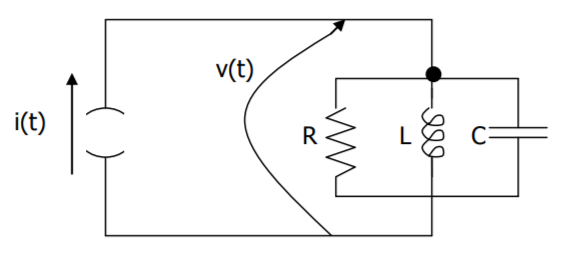
\includegraphics[scale=0.75]{04-FuncionTransferenciaYSistemasEstables/circuito18.png}\\
	$R=6$\\
	$L=5$\\
	$C=1/30$
	
	Cuya E.D. es: $\displaystyle \;\;\;\; i(t)=\frac{v(t)}{R}+\frac{1}{L}\int_{0}^{t}v(t)+C \frac{dv(t)}{dt}$
	
	Halle $v(t)$ para un impulso de corriente (aplicando Transformada de Laplace). \\
	
	Para resolverlo, nos limitamos a transformar y reemplazar los datos que nos dan:
	
	$\displaystyle I(s)=\frac{1}{R} V(s)+\frac{1}{L}\frac{V(s)}{s}+CsV(s)-\cancelto{0}{cv(0)}$
	
	La $i(t)$ no es otra que la función impulso (el enunciado dice un \underline{impulso} de corriente). Entonces $I(s)=1$
	
	$\displaystyle 1=V(s)\left(\frac{1}{R}+\frac{1}{Ls}+Cs\right)=V(s)\left(\frac{RLCs^2+Ls+R}{RLs}\right)\rightarrow V(s)=\frac{RLs}{RLCs^2+Ls+R}$
	
	Reemplazando los valores del ejercicio: $\displaystyle V(s)=\frac{30s}{s^2+5s+6}$
	
	Aplicando fracciones simples: $\displaystyle V(s)= \frac{-60}{s+2}+\frac{90}{s+3}$
	
	Por último, antitransformando: \fcolorbox{black}{yellow}{$v(t)=-60e^{-2t}+90e^{-3t}$}
	
	
\end{document}
 